% !TeX program=pdflatex
% !BIB program=biber
%
% NLDL full paper - compile: pdflatex -> biber -> pdflatex -> pdflatex
% Review mode (anonymized + line numbers) is the class default.
% Before submission: replace the placeholder \paperID with the OpenReview ID.
\documentclass[fullpaper]{nldl}

\paperID{0000}% <- replace with the OpenReview submission number
\vol{V}

%% Math
\usepackage{mathtools}

%% Figures
\usepackage{graphicx}
\graphicspath{{figs/}}

%% Tables
\usepackage{booktabs}

%% Required by the class's appendix setup
\usepackage{algorithm}
\usepackage{algorithmic}

%% Units (upright micro sign)
\usepackage{textcomp}
\newcommand{\uA}{\,\textmu A}
\newcommand{\um}{\,\textmu m}

%% References
\addbibresource{refs.bib}

%% Links
\usepackage{hyperref}
\usepackage{url}
\hypersetup{
  pdfusetitle,
  colorlinks,
  linkcolor = BrickRed,
  citecolor = NavyBlue,
  urlcolor  = Magenta!80!black,
}

\title{Digital Twinning of Neural Organoids with Resonant Reservoir Networks}
% Camera-ready only: replace with real authors and affiliations.
\author[1]{Anonymous Author}
\affil[1]{Anonymous Institution}

\begin{document}
\maketitle

\begin{abstract}
Neural organoids interfaced with microelectrode arrays (MEAs) are a candidate substrate for biological computing, but working with a living culture requires models of what that culture is doing: which sites drive which, and a simulator that reproduces the culture's dynamics when the tissue is not on the bench. We present a pipeline that produces both from single recording sessions of the open shell MEA dataset of hiPSC-derived neural organoids under electrical neuromodulation. Point-process generalised linear models recover directed effective connectivity on the three-dimensional shell geometry and show it is stimulation-dependent: raising the stimulation current from 5\uA{} to 30\uA{} doubles the number of significant couplings (23 to 46). Each organoid state is then fitted with an interpretable digital twin: a resonant reservoir network of fifteen damped resonators on two interleaved golden-ratio frequency ladders, read out through a doubly stochastic burst process and fitted with the many-objective evolutionary algorithm NSGA-III against five envelope-level objectives. Across sixteen organoid states the twins reproduce population rate (median absolute error 4\%), rate distribution, and spectral profile, and a teacher-forced variant tracks held-out activity with a median correlation of 0.92; a permutation-calibrated spectral test keeps the twins from reporting oscillations the data do not support.
\end{abstract}

\section{Introduction}
\label{sec:intro}

Organoid intelligence refers to the use of living neurons in vitro for information processing~\citep{huang2022shell,acha2026neuromodulation}. Cultures of neurons derived from human induced pluripotent stem cells (hiPSCs) are stimulated electrically through a microelectrode array (MEA), and exhibit forms of learning and plasticity that can be manipulated at the level of individual stimulation channels.

Reservoir computing is a framework for using the dynamics of a fixed, high-dimensional, nonlinear recurrent system for computation, training only a linear readout on the system's state~\citep{jaeger2001echo,maass2002realtime}. The input signal is expanded nonlinearly into a higher-dimensional state space, and only the output weights are fitted, typically by ridge regression; training therefore reduces to a convex problem and requires no gradient propagation through the recurrent dynamics. Two properties make a system a reservoir: \emph{fading memory}, so that the influence of past inputs decays and the state is a well-defined function of recent input history rather than of initial conditions, and a \emph{separation property}, so that distinct input histories drive distinct states. Because the reservoir itself is never trained, biological substrates such as neural organoids are natural candidates: synaptic and membrane time constants provide the required fading memory, and cultures are richly recurrently connected.

MEAs record electrical signals from, and deliver stimulation to, neural cultures. Conventional MEA plates are planar, designed for monolayer cultures, so contact with a three-dimensional organoid is limited to the small area where it rests on the plate. \Citet{huang2022shell} addressed this with a self-folding shell MEA designed by analogy to EEG caps: SU-8 bilayer leaflets carrying PEDOT:PSS-coated electrodes fold around the organoid, with the fold angle set by bilayer thickness and UV exposure and tuned to organoids of 400--600\um. Recording the same organoid through shell and planar MEAs simultaneously, the shell electrodes detected roughly four times as many spikes, at a higher signal-to-noise ratio. The shell geometry therefore places electrodes at known, non-degenerate positions distributed over the organoid surface---a precondition for resolving connectivity spatially and for stimulating specific regions.

Connectivity in an organoid is not uniform: stimulation at one electrode drives activity at some sites and not others. Learning this directed influence between electrodes makes plasticity targetable---connections that exist can be strengthened or weakened deliberately, while unconnected pairs act as controls. Point-process generalised linear models (PP-GLMs) compute this directed influence from recorded spike trains~\citep{truccolo2005point,pillow2008spatiotemporal}. Each unit's firing rate is modelled as the exponential of a sum of contributions: a baseline, the stimulus, the unit's own recent spikes, and the recent spikes of every other recorded unit, each weighted over a range of lags. The advantage over pairwise correlation is that these terms compete to explain the same spikes. Cultures burst synchronously, so correlation reports coupling between almost all pairs, whereas the PP-GLM's history term absorbs a unit's own bursting and leaves the coupling weights near zero unless a genuine directed effect remains. Because unrecorded neurons supplying common input cannot be represented, the recovered edges are effective rather than anatomical connections.

This paper presents a pipeline that turns one recording session of an organoid into two models of that organoid: a directed connectivity map and a generative digital twin. Its contributions are (i)~state-resolved directed connectivity on the shell geometry, showing that the effective network densifies with stimulation intensity (Sec.~\ref{sec:res-conn}); (ii)~an interpretable twin architecture---a resonant reservoir network with a doubly stochastic burst readout---whose parameters are fitted by many-objective evolution under a permutation-calibrated test that keeps spectral claims honest (Sec.~\ref{sec:methods-twin}); and (iii)~an evaluation across sixteen organoid states from three organoids, with a detailed case study of one state (Sec.~\ref{sec:res-case}).

\section{Related work}
\label{sec:related}

Reservoir computing originates with echo state networks~\citep{jaeger2001echo} and liquid state machines~\citep{maass2002realtime}, the latter explicitly framed as a model of computation in neural microcircuits. Our twin architecture follows \citet{kramer2025resonant}, who showed that recurrent networks built from lightly damped second-order resonators---resonant recurrent networks (RRNs)---are both performant and interpretable, in the sense that every hidden unit has an explicit centre frequency and damping, and that organising the centre frequencies as a golden-ratio ladder outperforms linear spacing. We repurpose this architecture: where \citet{kramer2025resonant} trains RRNs discriminatively on sequence tasks, we evolve one as a \emph{generative} model of a specific biological culture.

On the fitting side, \citet{sethi2026multiobjective} optimise spiking neural network models against several simultaneous objectives on oscillatory neural dynamics; we adopt the same philosophy---keep the objectives separate rather than collapsing them into one scalar loss---using the reference-point-based NSGA-III~\citep{deb2014nsga3}. For the connectivity map, we build on the point-process GLM framework of \citet{truccolo2005point}, applied to complete recorded populations by \citet{pillow2008spatiotemporal}. The substrate itself, hiPSC-derived organoids on self-folding shell MEAs, and the neuromodulation protocol that generated the dataset are due to \citet{huang2022shell} and \citet{acha2026neuromodulation}.

\section{Methods}
\label{sec:methods}

\subsection{Dataset and preprocessing}
\label{sec:methods-data}

\begin{figure*}[t]
  \centering
  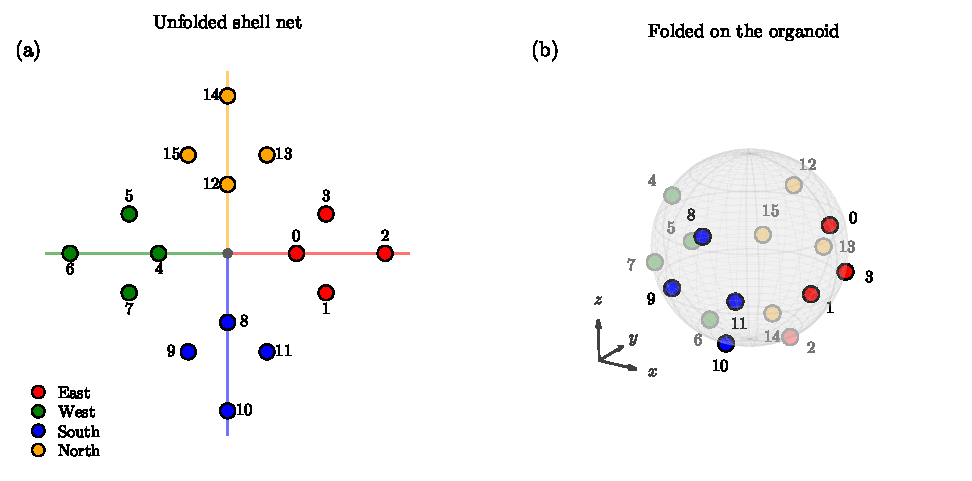
\includegraphics[width=0.92\textwidth]{shell_electrode_layout}
  \caption{Recording geometry of the 16-channel folded shell MEA. (a)~The unfolded device net: four leaflet arms (East, West, South, North) each carry four electrodes, indexed 0--15. (b)~The same electrodes after the shell is folded around the organoid, mapped onto a spherical surface by arc length from the net origin. Colours indicate the parent arm and match the arm colouring of the connectivity figures; this layout orients the electrode positions used in the 3D connectivity figures.}
  \label{fig:shell_layout}
\end{figure*}

All analyses were run on the open shell MEA dataset of hiPSC-derived neural organoids under electrical neuromodulation (DANDI:001336)~\citep{johnson2025dandi,acha2026neuromodulation}. Recordings are raw 30\,kHz electrode streams from self-folding shell MEAs~\citep{huang2022shell,acha2026neuromodulation}: sixteen channels for organoid BO14, recorded for eight minutes at each of seven stimulation intensities (5 to 60\uA), and three channels for organoids BO2 and SO1, covering seven ${\sim}90$\,s stimulation states and two spontaneous sessions of about five minutes, respectively. The sixteen recording sites tile the organoid surface as four four-electrode leaflet arms, as shown in Fig.~\ref{fig:shell_layout}. Each recording is treated as one \emph{organoid state}, and the pipeline produces, per state, a directed connectivity estimate and a fitted digital twin.

Spikes were detected per channel after decimating the stream to 10\,kHz and applying a fourth-order zero-phase Butterworth high-pass filter at 300\,Hz. The detection threshold was set at 4.5 times a robust noise estimate (the median absolute signal divided by 0.6745), applied to negative-going peaks with a 1.5\,ms refractory constraint; the estimate is taken from the median rather than the variance so that the spikes themselves do not inflate the threshold. Detected spikes were binned at 1\,ms for connectivity analysis, and summed across channels in 1\,s bins to form the population firing-rate envelope on which twinning operates. Channels contributing fewer than 50 spikes were excluded from the connectivity model.

\subsection{Directed connectivity}
\label{sec:methods-conn}

Directed connectivity was estimated with a point-process GLM of the form introduced above, implemented as one logistic regression per target channel on 1\,ms bins. With $n_j(t)\in\{0,1\}$ the spike indicator of channel $j$, the spiking probability of target channel $i$ is modelled as
\begin{equation}
  \label{eq:glm}
  p_i(t) = \operatorname{expit}\Bigl(\beta_{i0} + \sum_{j} \sum_{\ell=1}^{20} \beta_{ij}^{(\ell)}\, n_j(t-\ell)\Bigr),
\end{equation}
so a unit's own history ($j=i$) competes with the couplings, and the coupling from source $j$ to target $i$ is the summed lag profile $c_{j\to i}=\sum_{\ell}\beta_{ij}^{(\ell)}$. Fits used an L2 penalty on up to 60\,000 subsampled bins. Significance was assessed against a null in which each channel's spike train is independently circularly shifted, which preserves every rate and autocorrelation while destroying timing relations; only couplings exceeding the 95th percentile of the null distribution were kept as edges, and electrodes were ranked as drivers or receivers by summed outgoing and incoming coupling magnitude on the shell geometry.

\subsection{The resonant reservoir twin}
\label{sec:methods-twin}

The digital twin is a resonant reservoir network in the sense of \citet{kramer2025resonant}: a bank of $K=15$ damped second-order resonators operating on the 1\,s population-rate envelope ($F_s=1$\,Hz). Resonator $k$ holds state $x_k(t)$ with autoregressive coefficients set by its centre frequency $f_k$ and a shared damping $r$,
\begin{multline}
  \label{eq:ar2}
  x_k(t) = 2r\cos\bigl(\tfrac{2\pi f_k}{F_s}\bigr)\,x_k(t-1) - r^2\,x_k(t-2) \\
  + u(t) + \bigl[\mathbf{W}\,\operatorname{expit}(\cos\boldsymbol{\phi}(t-1))\bigr]_k + \xi_k(t),
\end{multline}
where $u(t)=a_d\sin(2\pi f_d t)$ is a parametric sinusoidal drive, $\xi_k\sim\mathcal{N}(0,\sigma^2)$ is state noise, and each resonator's instantaneous amplitude $\alpha_k(t)$ and phase $\phi_k(t)$ are reconstructed from consecutive states through the damped-oscillator relations. The poles $r\,e^{\pm i 2\pi f_k/F_s}$ are stable for any $f_k<F_s/2$ whenever $r<1$, and $r$ is itself evolvable up to near-critical values so that nodes can ring selectively with the data. The centre frequencies climb geometrically from 0.015 to 0.435\,Hz as two interleaved golden-ratio ladders---adjacent nodes a factor $\sqrt{\varphi}\approx1.27$ apart and alternate nodes exactly the golden ratio $\varphi$ apart---following \citepos{kramer2025resonant} finding that golden-ratio frequency organisation outperforms linear spacing. The resonators are sparsely coupled through their instantaneous phases on a fixed random skeleton (density 0.35) whose 74 nonzero weights $\mathbf{W}$ are free parameters, rescaled to an evolved spectral radius $\rho$. The twin runs autonomously: it is driven only by $u(t)$ and noise, never by the recording.

The population rate is produced by a doubly stochastic burst readout. The standardised mean resonator amplitude $z(t)$ acts as a latent excitability that modulates both the probability and the size of discrete burst events,
\begin{align}
  \label{eq:events}
  e(t) &\sim \operatorname{Bernoulli}\Bigl(\min\bigl(1,\; p_0\, e^{\kappa z(t)} \big/ \langle e^{\kappa z}\rangle\bigr)\Bigr),\\
  \label{eq:sizes}
  a(t) &= A\, e^{s\,g(t) + \beta z(t)} \big/ \bigl\langle e^{s g + \beta z}\bigr\rangle,
  \qquad g(t)\sim\mathcal{N}(0,1),
\end{align}
so event sizes are lognormal, and the normalisers make $p_0$ the mean event probability and $A$ the mean event size. Events decay geometrically over one to a few seconds and ride on a quiescent baseline $b$:
\begin{equation}
  \label{eq:readout}
  y(t) = b + \sum_{\tau\ge0} d^{\,\tau}\, e(t-\tau)\, a(t-\tau).
\end{equation}
One mechanism thus spans the observed phenotypes: sparse events over a low baseline reproduce the aperiodic bursting and near-flat rate spectrum of the stimulated states, while dense, strongly modulated events recover a smooth rhythmic envelope, with the reservoir supplying the temporal structure in both regimes. Every simulation discards an initial washout before anything is evaluated---at least 90\,s, stretched to four time constants of the resonator poles for lightly damped candidates and capped at 600\,s---so that equilibration from the zero state never reaches the objectives.

\subsection{Many-objective fitting and model selection}
\label{sec:methods-fit}

Twin parameters (thirteen global parameters and the 74 recurrent weights) were fitted with NSGA-III~\citep{deb2014nsga3}, following the multi-objective fitting methodology of \citet{sethi2026multiobjective}. Each candidate is simulated for $B=15$ independent noise realisations, and each objective is the root-mean-square error over those trials normalised by its target $m^{*}$,
\begin{equation}
  \label{eq:objective}
  F_m = \frac{1}{|m^{*}|}\sqrt{\frac{1}{B}\sum_{b=1}^{B}\bigl(\hat{m}^{(b)} - m^{*}\bigr)^{2}},
\end{equation}
with the composite error defined as $\smash{\sqrt{\tfrac{1}{5}\sum_m F_m^2}}$. Five objectives are kept separate: population firing rate; dominant-oscillation mismatch; spectral containment (the overlap of normalised band power spectra); a synchronisation loss, in which the same reservoir is instead driven by the organoid envelope and a ridge readout of its resonator amplitudes, fitted on the first 70\% of the recording, must track the envelope on the held-out remainder; and the Wasserstein-1 distance between organoid and twin rate distributions, which penalises twins that match the mean but not the bursting.

A dominant oscillation is only accepted if the smoothed band spectrum has an interior peak whose prominence above a median-filtered local background exceeds the 95th percentile of the same statistic on surrogates in which the envelope bins are randomly shuffled---an exact permutation test that preserves the amplitude distribution while destroying all timing structure. Monotone or merely tilted $1/f$ spectra are therefore reported explicitly as having \emph{no} dominant oscillation, and the oscillation objective then penalises spurious twin peaks at the same calibrated threshold. The search ran 25 generations with population 50 under Das--Dennis reference directions, simulated binary crossover, and polynomial mutation, with all noise realisations shared across candidates (common random numbers). The twin is selected from the pooled nondominated front by excluding, within 25\% of the minimum composite error, members with spurious oscillations, and taking the lowest composite among the remainder. Finally, for subjects with multiple sessions, targets, twin fidelity, twin parameters, and connectivity statistics were tracked longitudinally across sessions.

\section{Results}
\label{sec:results}

\begin{figure*}[tb]
  \centering
  \begin{subfigure}[t]{0.42\textwidth}
    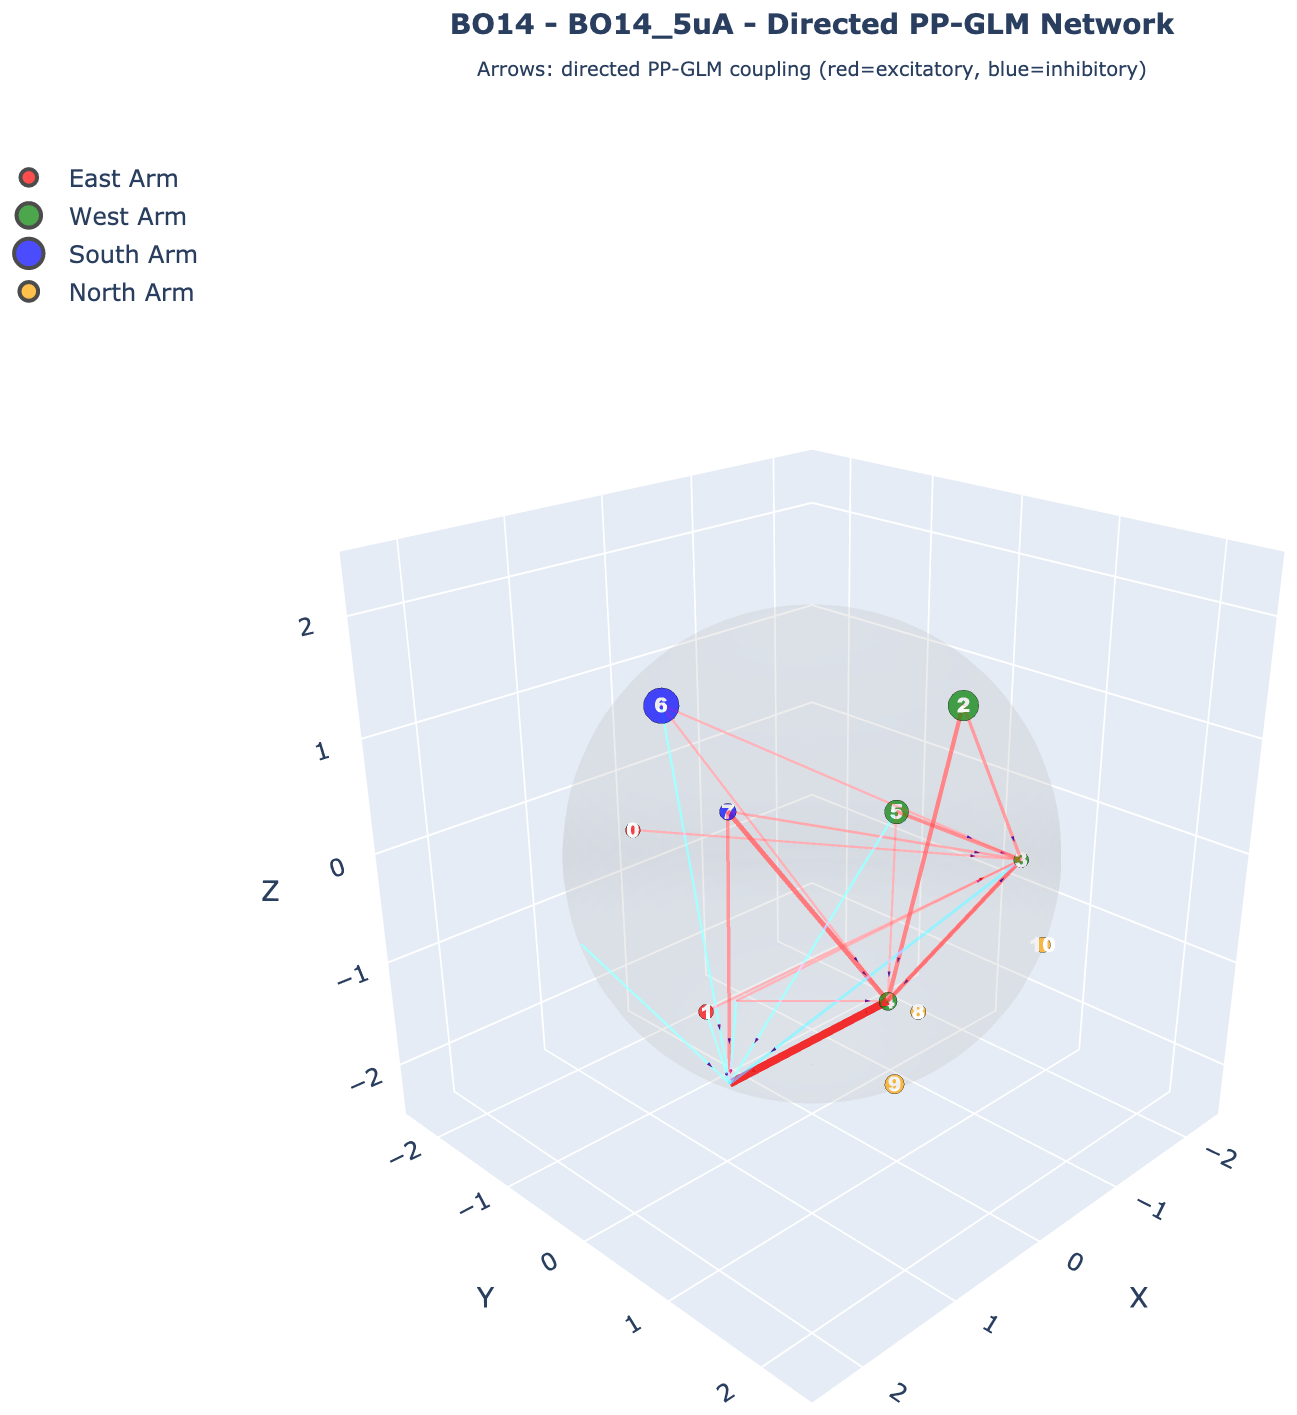
\includegraphics[width=\linewidth]{fig1a_ppglm_5uA}
    \caption{Stimulation at 5\uA: 23 edges.}
    \label{fig:ppglm-5}
  \end{subfigure}
  \hfill
  \begin{subfigure}[t]{0.42\textwidth}
    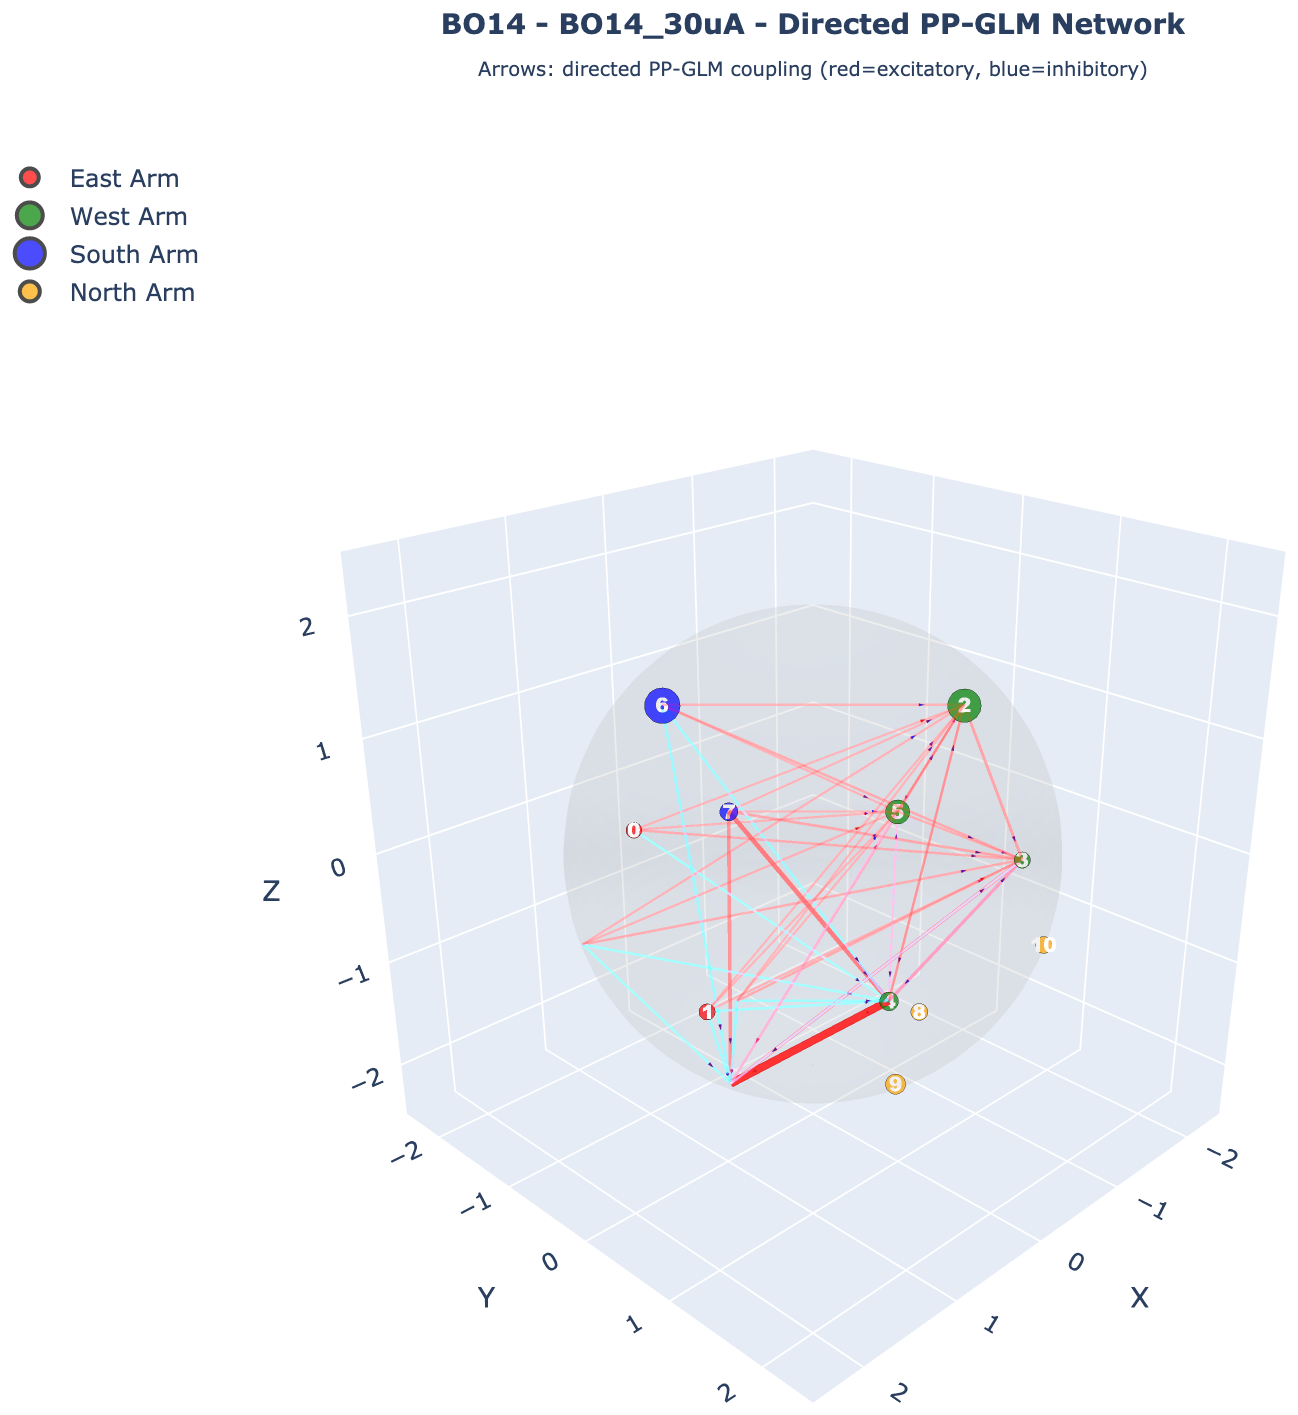
\includegraphics[width=\linewidth]{fig1b_ppglm_30uA}
    \caption{Stimulation at 30\uA: 46 edges.}
    \label{fig:ppglm-30}
  \end{subfigure}
  \caption{Directed PP-GLM connectivity for organoid BO14 on the shell geometry. Nodes are electrodes at their positions on the folded shell MEA, coloured by leaflet arm; node size scales with total coupling. Arrows are couplings exceeding the 95th percentile of the circular-shift null (red excitatory, blue inhibitory), with width scaled by coupling magnitude. From 5\uA{} to 30\uA{} the edge count doubles from 23 to 46 and the mean absolute coupling across channel pairs rises from 0.49 to 0.69, while the null threshold is nearly unchanged (0.366 vs.\ 0.360): the recovered network is state-dependent rather than fixed.}
  \label{fig:ppglm}
\end{figure*}

\subsection{Connectivity is stimulation-dependent}
\label{sec:res-conn}

Fig.~\ref{fig:ppglm} shows the directed PP-GLM network of organoid BO14 (eleven channels passed the 50-spike inclusion threshold) at two stimulation intensities. Raising the current from 5\uA{} to 30\uA{} doubles the number of significant couplings from 23 to 46, and the mean absolute coupling across all channel pairs rises from 0.49 to 0.69. The circular-shift null threshold is nearly identical in the two states (0.366 vs.\ 0.360), so the densification is a property of the recovered network, not of the significance test. The strongest couplings link the same electrode pair (channels 2 and 6) in both states, and the same electrodes recur as the dominant drivers, so intensity appears to recruit additional couplings around a stable core rather than rewiring the network wholesale. For plasticity experiments this is the useful regime: edges that exist can be targeted, and their intensity dependence gives a dial.

\begin{figure*}[tb]
  \centering
  \begin{subfigure}[t]{0.49\textwidth}
    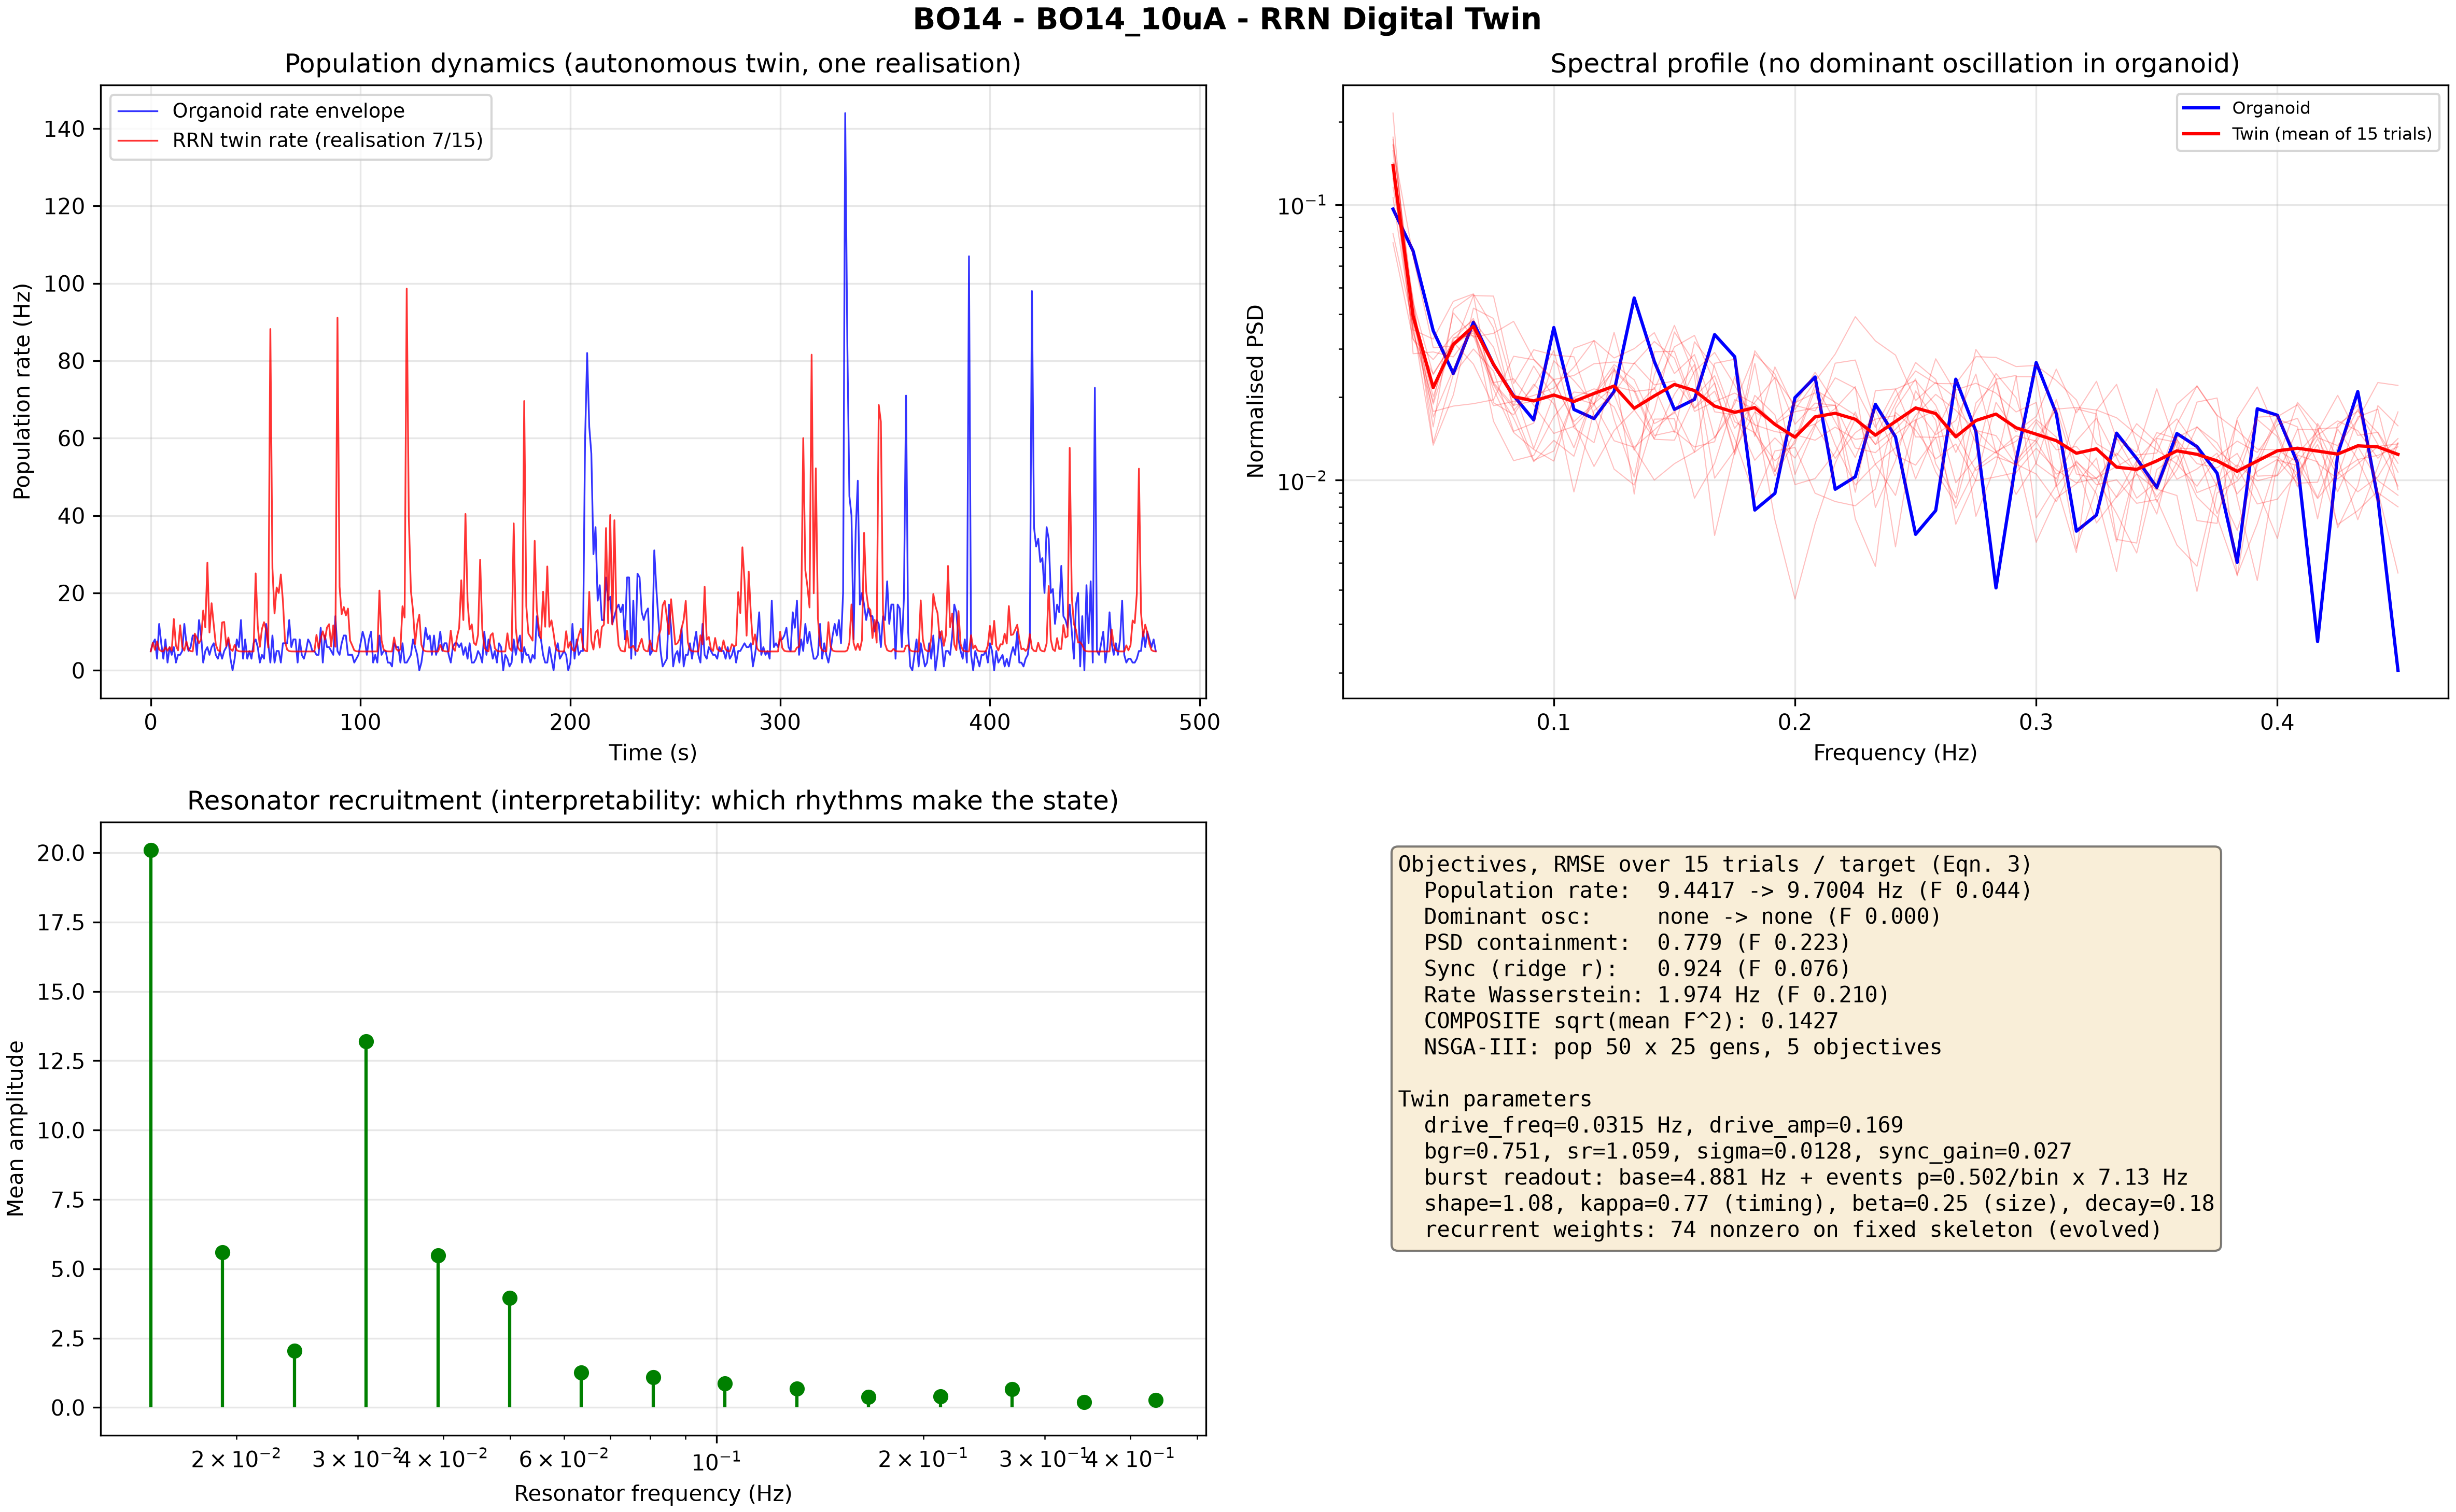
\includegraphics[width=\linewidth]{fig2a_twin_BO14_10uA}
    \caption{BO14 at 10\uA{} (eight-minute state).}
    \label{fig:twin-bo14}
  \end{subfigure}
  \hfill
  \begin{subfigure}[t]{0.49\textwidth}
    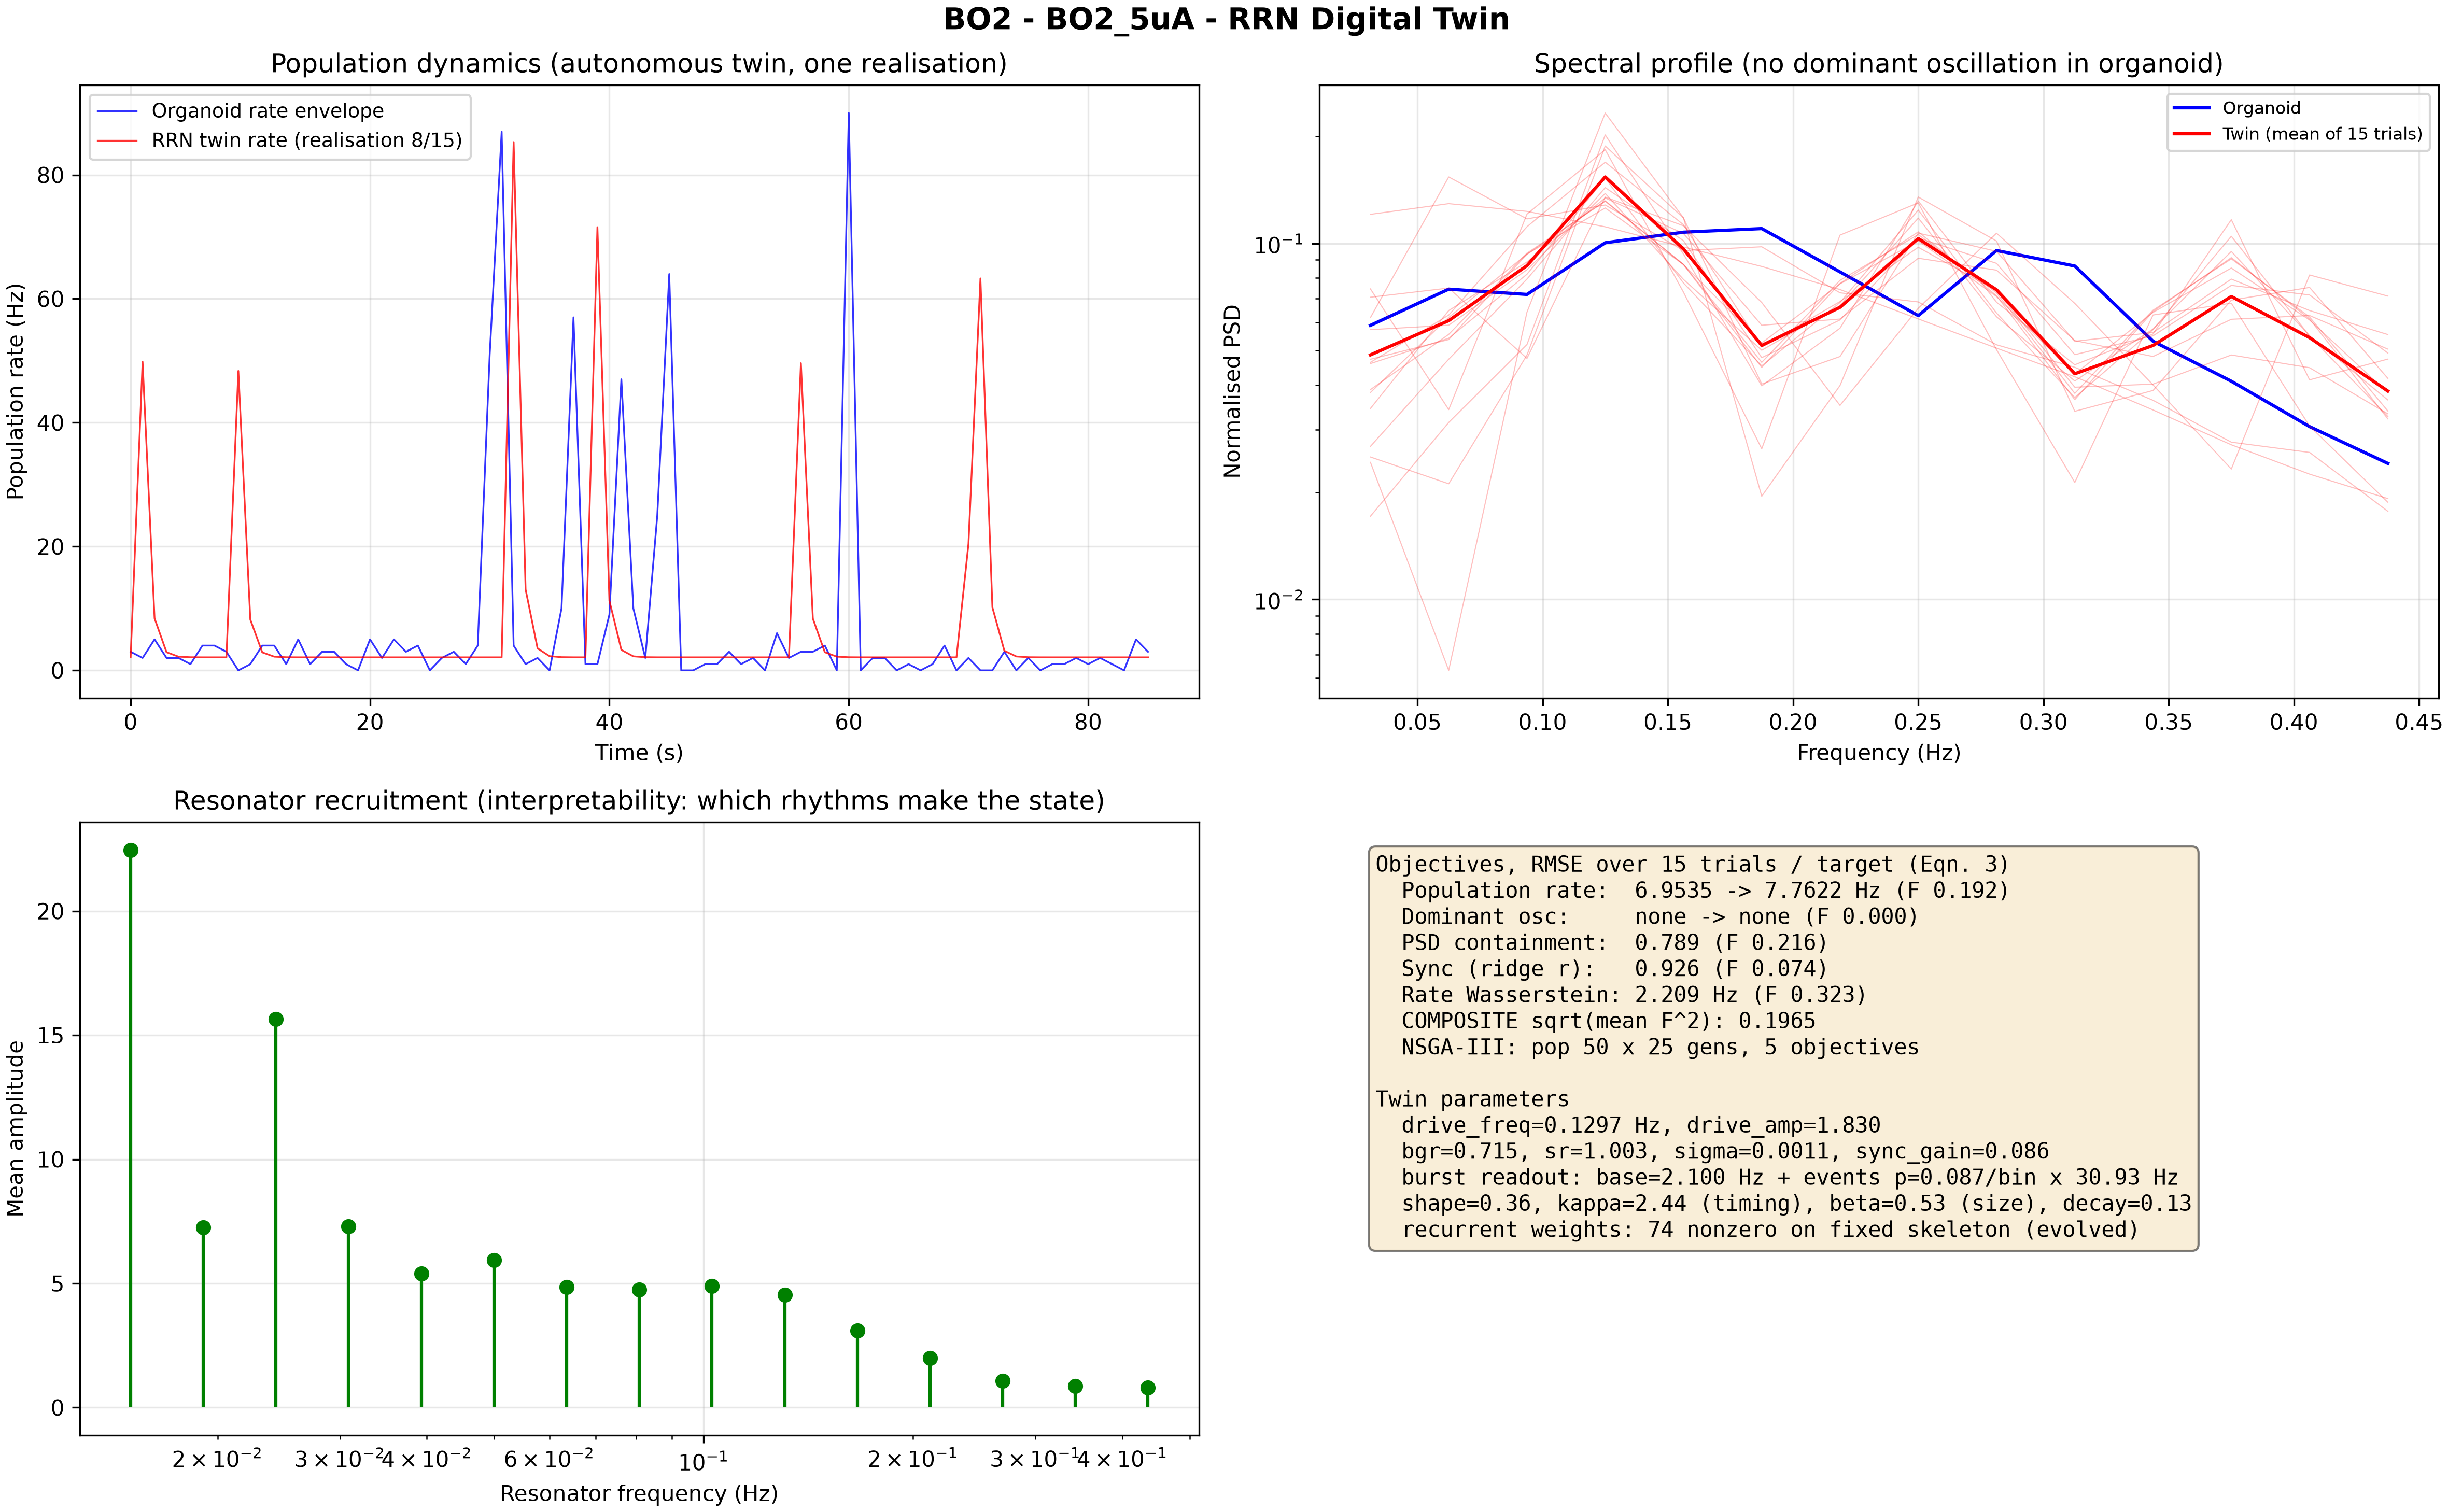
\includegraphics[width=\linewidth]{fig2b_twin_BO2_5uA}
    \caption{BO2 at 5\uA{} (${\sim}90$\,s state).}
    \label{fig:twin-bo2}
  \end{subfigure}
  \caption{Resonant reservoir twins of two organoid states. Within each panel: the organoid population-rate envelope against one autonomous twin realisation (top left); normalised band power spectra, with the fifteen twin realisations in light red and their mean in bold---neither state has an accepted dominant oscillation (top right); the mean amplitude of each of the fifteen resonators, showing which rhythms carry the state (bottom left); and the five NSGA-III objectives with the selected parameters (bottom right). The composite error is 0.14 for (a), with target rate 9.44\,Hz against 9.70\,Hz achieved and held-out synchronisation $r=0.92$, and 0.20 for (b), with 6.95\,Hz against 7.76\,Hz and $r=0.93$.}
  \label{fig:twins}
\end{figure*}

\subsection{Twins across organoids and states}
\label{sec:res-twins}

All sixteen organoid states (seven BO14 intensities, seven BO2 intensities, two SO1 spontaneous sessions) were twinned with the same architecture and search settings; Appendix~\ref{app:states} tabulates every fit. Composite errors range from 0.14 to 0.37. The autonomous twins match the target population rate with a median absolute error of 4\% (eleven of sixteen states within 8\%), and the teacher-forced synchronisation check reaches a median held-out correlation of $r=0.92$ (range 0.61--0.97). In no state does the twin report an oscillation that the permutation test does not also find in the organoid.

Fig.~\ref{fig:twins} shows two states with deliberately different characters. The BO14 state (Fig.~\ref{fig:twins}a) is an eight-minute recording with dense, irregular bursting over a raised baseline; the fitted readout sits in the dense-event regime (mean event probability 0.50 per bin, mean event size 7.1\,Hz over a 4.9\,Hz baseline, as listed in the panel). The BO2 state (Fig.~\ref{fig:twins}b) is a ${\sim}90$\,s recording whose envelope is a handful of large, isolated population bursts on a nearly silent background; the same mechanism moves to the sparse regime (event probability 0.09 per bin, mean event size 31\,Hz over a 2.1\,Hz baseline). One readout family spans both phenotypes, and the resonator-recruitment panels make the twins interpretable: in both states the mass sits in the two slowest ladder rungs near 0.015--0.03\,Hz, identifying the minute-scale envelope fluctuations that carry the state. Neither organoid has a statistically significant dominant oscillation, and neither twin claims one.

\subsection{Case study: BO14 at 20\texorpdfstring{\uA}{ uA}}
\label{sec:res-case}

\begin{figure*}[tb]
  \centering
  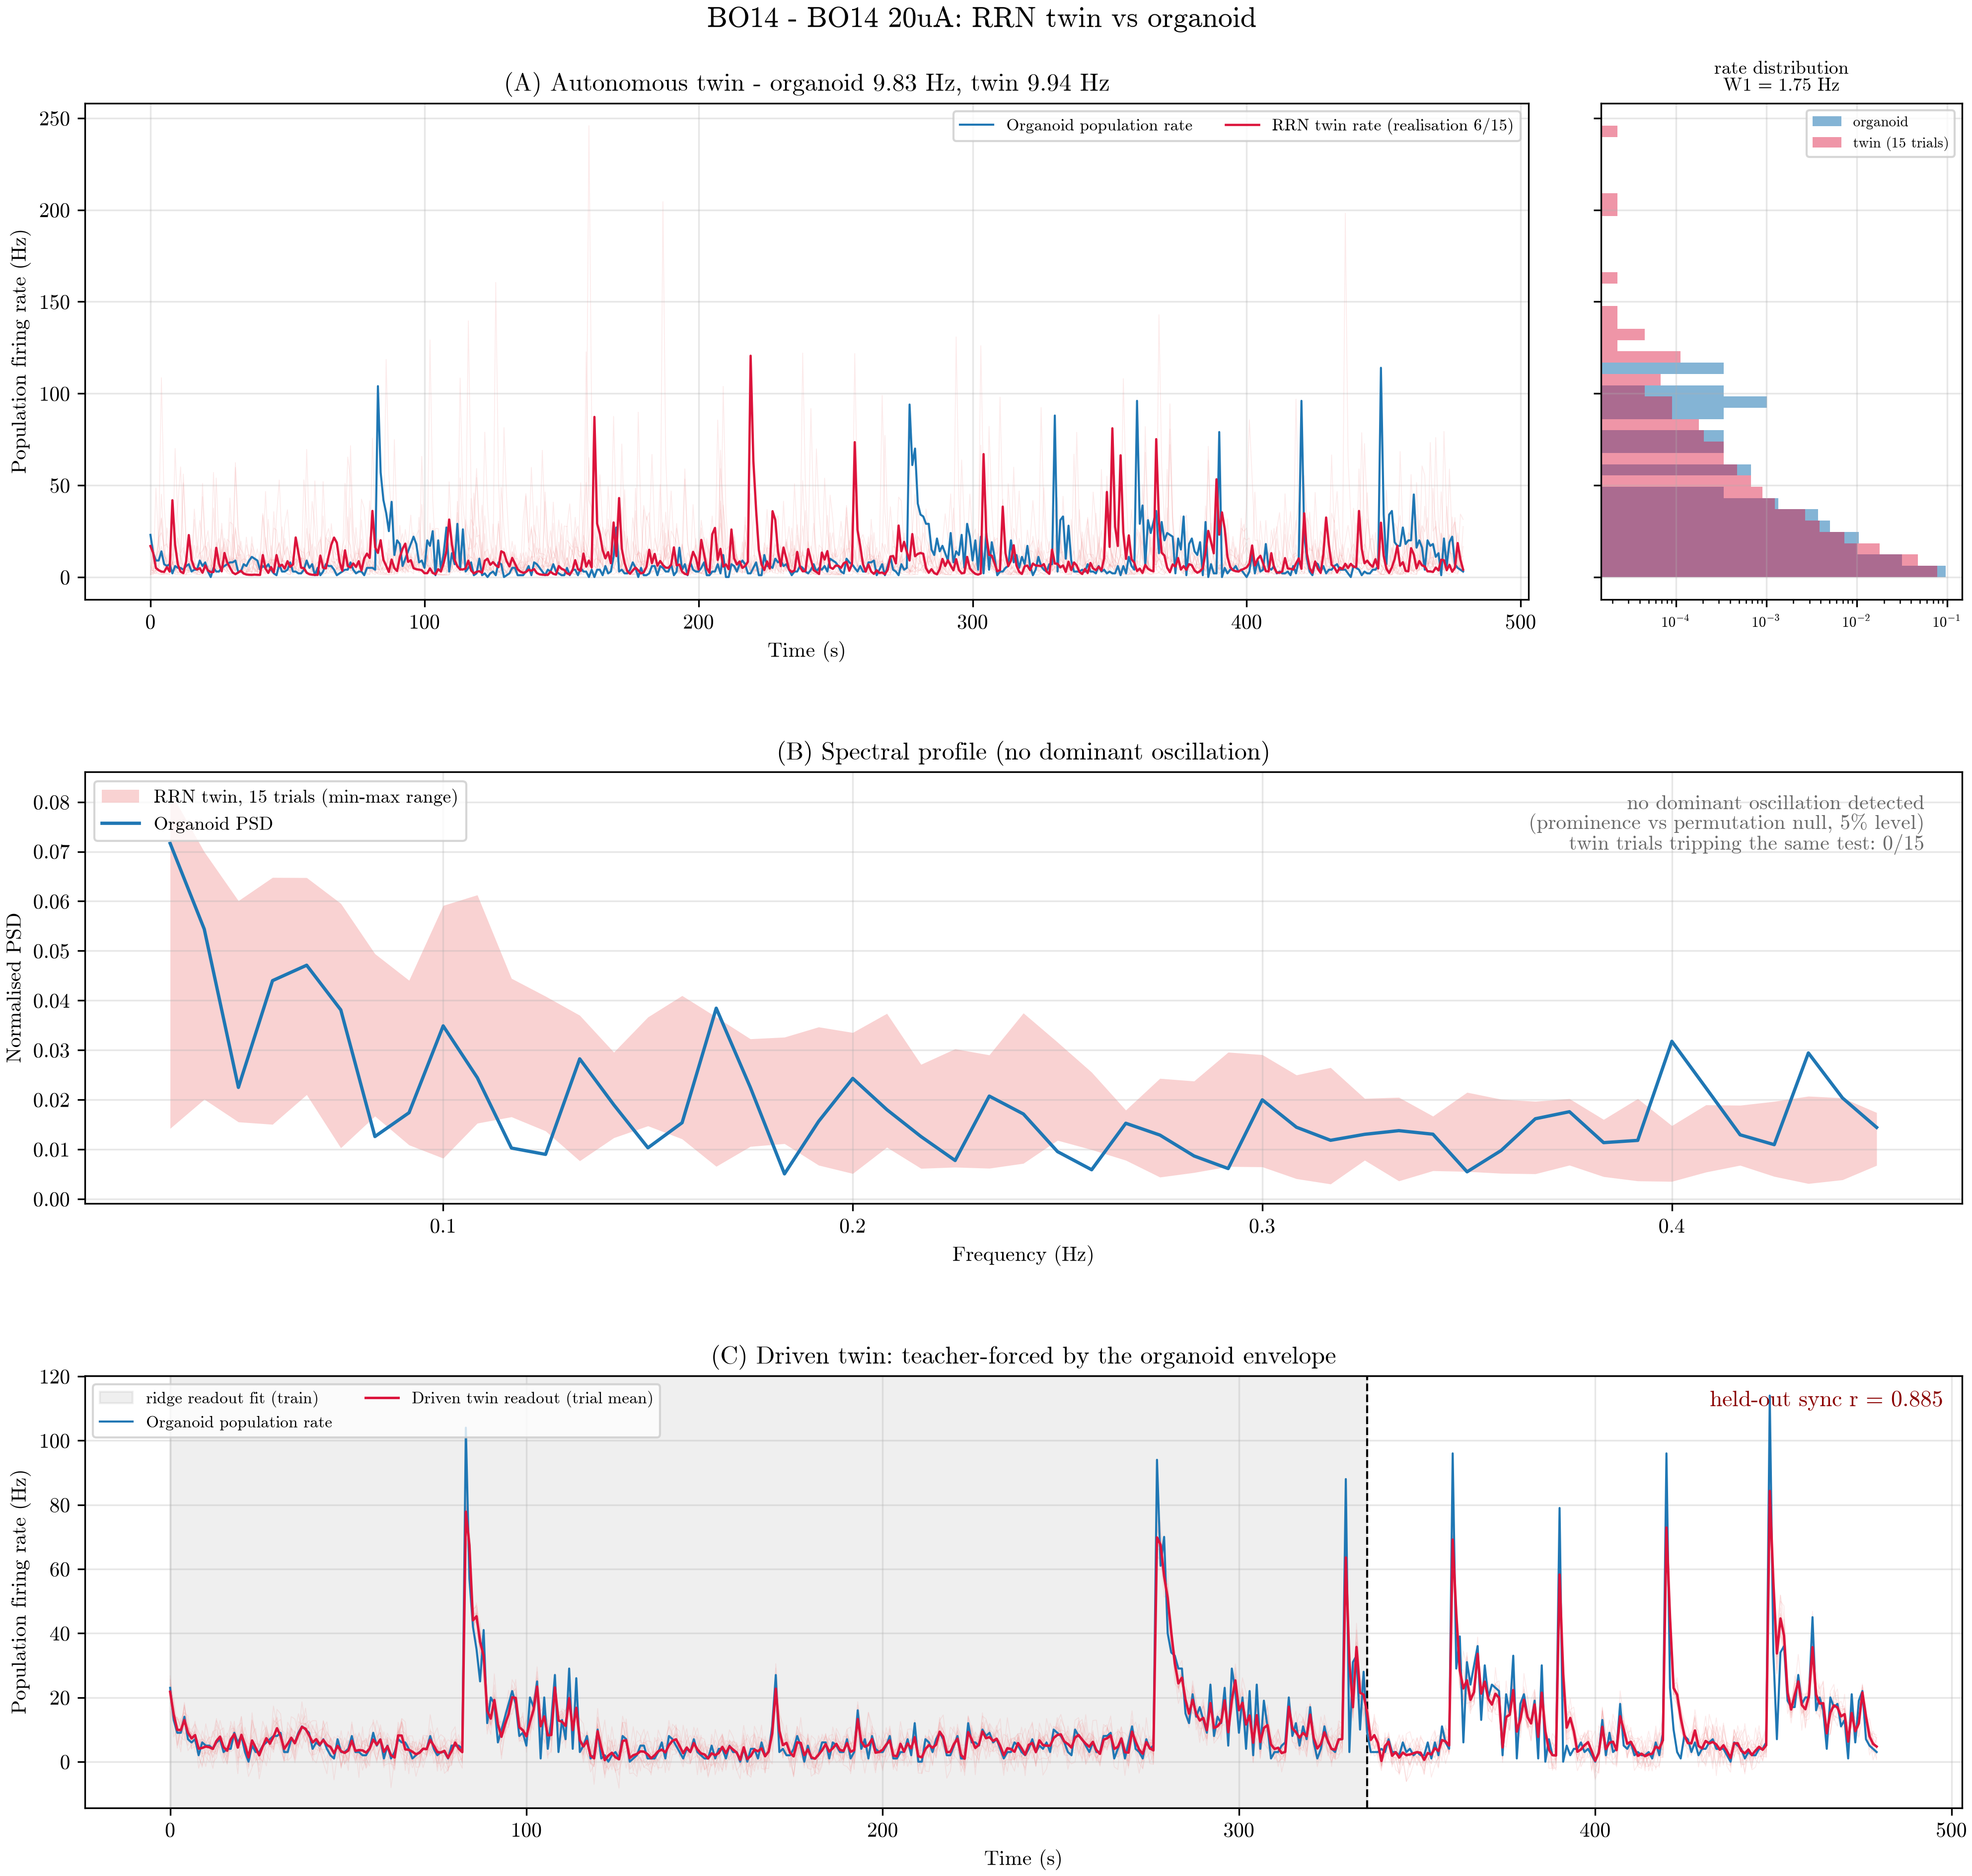
\includegraphics[width=0.86\textwidth]{fig3_activity_BO14_20uA}
  \caption{The BO14 20\uA{} twin in detail. (A)~Autonomous twin: one noise realisation of the fitted twin against the organoid population-rate envelope (organoid 9.83\,Hz, twin 9.94\,Hz); the marginal panel compares the rate distributions (Wasserstein distance 1.75\,Hz). (B)~Spectral profile: the organoid power spectrum on top of the min--max range over fifteen twin trials; neither organoid nor twin shows a dominant oscillation under the permutation test. (C)~Driven twin: the same reservoir teacher-forced by the organoid envelope tracks the recording through a ridge readout of its resonator amplitudes; the segment right of the dashed split is held out ($r=0.885$).}
  \label{fig:activity}
\end{figure*}

\begin{table}[tb]
  \centering
  \caption{Fitted twin of BO14 at 20\uA: parameters (top) and achieved fidelity (bottom). Rates in Hz; $p_0$ and $d$ are per 1\,s envelope bin.}
  \label{tab:params}
  \small
  \begin{tabular}{@{}lr@{}}
    \toprule
    Parameter & Value \\
    \midrule
    \multicolumn{2}{@{}l}{\emph{Reservoir}} \\
    \quad resonators $K$ (two golden ladders) & 15 \\
    \quad centre frequencies (Hz) & 0.015--0.435 \\
    \quad damping $r$ & 0.744 \\
    \quad spectral radius $\rho$ & 0.925 \\
    \quad state noise $\sigma$ & 0.072 \\
    \quad recurrent weights (evolved) & 74 \\
    \multicolumn{2}{@{}l}{\emph{Drive}} \\
    \quad frequency $f_d$ (Hz) & 0.043 \\
    \quad amplitude $a_d$ & 0.029 \\
    \multicolumn{2}{@{}l}{\emph{Readout}} \\
    \quad baseline $b$ (Hz) & 1.16 \\
    \quad event probability $p_0$ & 0.887 \\
    \quad event size $A$ (Hz) & 7.26 \\
    \quad lognormal shape $s$ & 1.19 \\
    \quad timing gain $\kappa$ & 0.330 \\
    \quad size gain $\beta$ & 0.172 \\
    \quad kernel decay $d$ & 0.319 \\
    \quad sync gain $g$ (driven mode) & 0.149 \\
    \midrule
    composite normalised RMSE & 0.145 \\
    rate, target $\to$ twin (Hz) & $9.83 \to 9.94$ \\
    dominant osc., organoid / twin & none / none \\
    spectral containment & 0.758 \\
    held-out synchronisation $r$ & 0.885 \\
    rate Wasserstein-1 (Hz) & 1.75 \\
    \bottomrule
  \end{tabular}
\end{table}

\begin{figure}[tb]
  \centering
  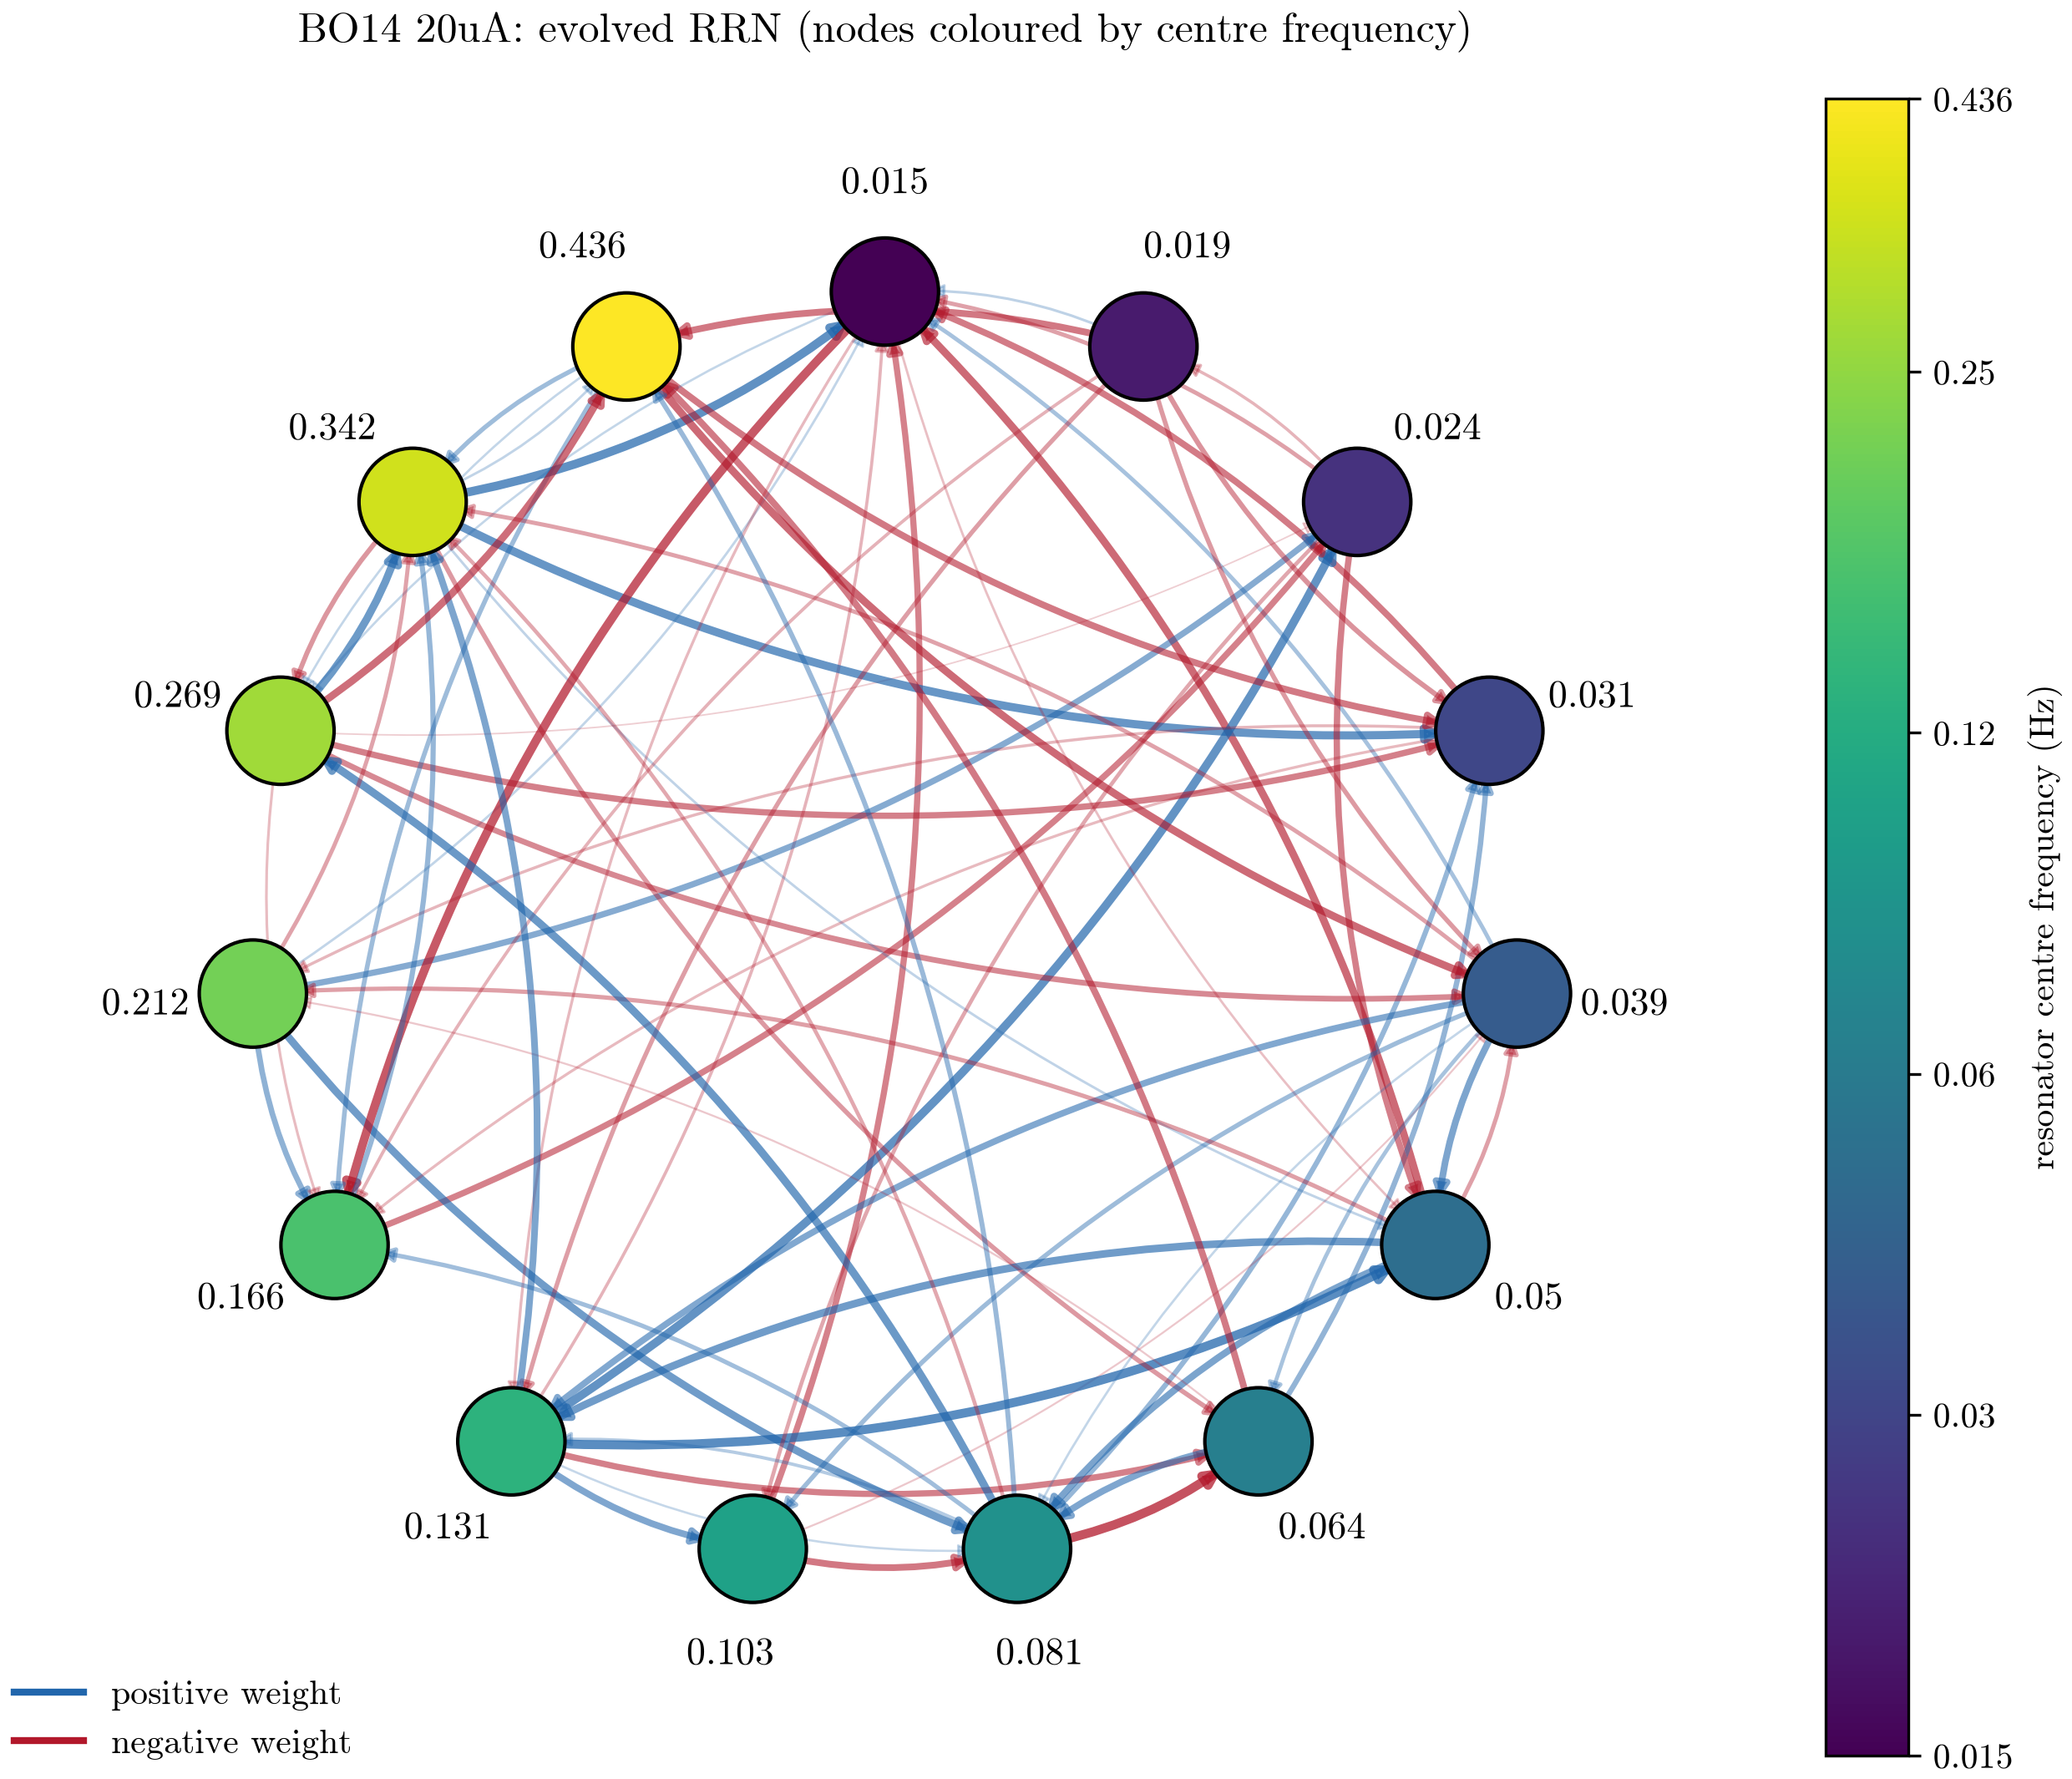
\includegraphics[width=\linewidth]{fig4_reservoir_BO14_20uA}
  \caption{The evolved reservoir behind Fig.~\ref{fig:activity}: fifteen damped resonators whose centre frequencies (node colour, log scale) climb from 0.015 to 0.435\,Hz as two interleaved golden-ratio ladders, coupled by the 74 evolved recurrent weights (blue positive, red negative; width proportional to magnitude).}
  \label{fig:reservoir}
\end{figure}

Fig.~\ref{fig:activity} examines the state shown throughout the rest of the paper, BO14 at 20\uA, with the corresponding parameters and fidelity in Table~\ref{tab:params} and the evolved reservoir in Fig.~\ref{fig:reservoir}. The autonomous twin matches the target rate within 1.1\% (9.83\,Hz target, 9.94\,Hz achieved; the rate objective alone is $F=0.034$) and reproduces the burst-dominated rate distribution to a Wasserstein-1 distance of 1.75\,Hz (Fig.~\ref{fig:activity}A). Spectrally, the organoid's envelope has no statistically significant dominant oscillation, and the twin agrees: not one of the fifteen twin trials produces a spurious peak at the calibrated threshold, and the organoid spectrum sits largely inside the twins' min--max band (containment 0.758; Fig.~\ref{fig:activity}B). When the same reservoir is teacher-forced by the organoid envelope, a ridge readout of its resonator amplitudes tracks the held-out final 30\% of the recording at $r=0.885$ (Fig.~\ref{fig:activity}C), evidence that the evolved dynamics carry usable temporal structure rather than merely matching summary statistics.

Table~\ref{tab:params} also shows where in the readout's regime space the search landed: a dense-event solution ($p_0=0.887$ events per bin) with a heavy lognormal size spread ($s=1.19$) over a low 1.16\,Hz baseline. This state's bursting is expressed through amplitude variability at nearly every bin, in contrast to the sparse large-event solution found for BO2 at 5\uA{} (Sec.~\ref{sec:res-twins}); the two regimes are endpoints of the same four-parameter mechanism, not different models. The evolved recurrent matrix (Fig.~\ref{fig:reservoir}) is balanced---35 positive and 39 negative weights---with a subcritical spectral radius of 0.925, and the moderate damping $r=0.744$ makes the resonators broadband rather than sharply tuned, consistent with the aperiodic character of the state.

\section{Discussion and conclusion}
\label{sec:discussion}

\textbf{Interpretability.} Every twin parameter has physical meaning and units: a baseline in Hz, an event probability per second, an event size in Hz, a damping and a spectral radius, and fifteen centre frequencies fixed on a golden-ratio ladder. A reviewer can read Table~\ref{tab:params} and know what the model claims about the culture---roughly one burst event per second, seven-hertz average size, heavy size tail, no preferred rhythm---and the resonator-recruitment profile identifies which timescales carry each state. This is the sense in which the RRN of \citet{kramer2025resonant} is interpretable, inherited here by a generative model of a specific biological preparation.

\textbf{Honest negatives.} An unconstrained spectral objective invites twins that invent rhythms, and peak heuristics on $1/f$-tilted spectra invite the analyst to report oscillations that are not there. The permutation-calibrated test controls both sides at once: none of the sixteen organoid states in this dataset supports a dominant envelope oscillation at the 5\% level, and none of the sixteen twins claims one. We consider the resulting negatives---``no dominant oscillation''---as informative as the fits themselves.

\textbf{Limitations.} PP-GLM edges are effective, not anatomical: unrecorded common input cannot be represented, and BO2 and SO1 expose only three channels, too few for spatial claims. The twin operates on the 1\,s population envelope, so it models the culture's collective burst dynamics, not spike-level or channel-level structure. The weakest fits are informative about failure modes: the largest rate miss (14\% for BO14 at 30\uA) coincides with a nonstationary session whose late burst cluster the stationary twin averages over, and the weakest held-out synchronisation ($r=0.61$, BO2 at 20\uA) is a ${\sim}90$\,s state whose held-out tail contains almost no burst events to track.

\textbf{Outlook.} The two models are complementary in a closed-loop setting: the connectivity map says where to stimulate, and the twin provides an unlimited in-silico copy of the state for protocol design before the wet experiment. Because twin parameters are physical, tracking them longitudinally turns culture development and plasticity into trajectories in an interpretable parameter space---an inexpensive readout of whether a targeted intervention changed the culture, and by how much.

\printbibliography

\appendix

\section{Twin fidelity for all sixteen states}
\label{app:states}

Table~\ref{tab:allstates} lists every organoid state and its fitted twin: target and achieved population rate, held-out synchronisation correlation, Wasserstein-1 distance between rate distributions, and composite normalised RMSE (Eq.~\ref{eq:objective}). The two SO1 rows are the two spontaneous sessions in chronological order. All sixteen states were fitted with the same architecture, objectives, and search budget; no state is excluded.

\begin{table}[tb]
  \centering
  \caption{Twin fidelity across all sixteen organoid states. Rates and $W_1$ in Hz.}
  \label{tab:allstates}
  \resizebox{\linewidth}{!}{%
  \begin{tabular}{@{}llrrrrr@{}}
    \toprule
    Organoid & State & Target & Twin & $r$ & $W_1$ & RMSE \\
    \midrule
    BO14 & 5\uA  & 9.71 & 8.85 & 0.81 & 1.32 & 0.151 \\
    BO14 & 10\uA & 9.44 & 9.70 & 0.92 & 1.97 & 0.143 \\
    BO14 & 20\uA & 9.83 & 9.94 & 0.89 & 1.75 & 0.145 \\
    BO14 & 30\uA & 9.64 & 8.28 & 0.95 & 3.40 & 0.211 \\
    BO14 & 40\uA & 9.86 & 10.32 & 0.93 & 1.71 & 0.145 \\
    BO14 & 50\uA & 9.18 & 9.26 & 0.90 & 2.36 & 0.219 \\
    BO14 & 60\uA & 8.19 & 8.08 & 0.92 & 2.34 & 0.178 \\
    BO2 & 5\uA  & 6.95 & 7.76 & 0.93 & 2.21 & 0.197 \\
    BO2 & 10\uA & 7.93 & 7.68 & 0.97 & 4.55 & 0.281 \\
    BO2 & 20\uA & 7.19 & 7.19 & 0.61 & 4.91 & 0.372 \\
    BO2 & 30\uA & 6.27 & 6.76 & 0.90 & 3.44 & 0.280 \\
    BO2 & 40\uA & 6.47 & 5.61 & 0.91 & 2.86 & 0.245 \\
    BO2 & 50\uA & 3.54 & 3.49 & 0.95 & 1.77 & 0.256 \\
    BO2 & 60\uA & 3.24 & 3.21 & 0.95 & 1.28 & 0.218 \\
    SO1 & spont.\ (i)  & 0.25 & 0.22 & 0.87 & 0.11 & 0.256 \\
    SO1 & spont.\ (ii) & 2.92 & 2.74 & 0.94 & 1.57 & 0.267 \\
    \bottomrule
  \end{tabular}}
\end{table}

\end{document}
